\documentclass{elsarticle}
\usepackage{geometry, graphicx}
\usepackage{xcolor, booktabs}
\usepackage{amsmath, amssymb}
\usepackage{subcaption, placeins}
\usepackage[title]{appendix}


\begin{document}


\begin{frontmatter}

\title{Calculation of grain boundary diffusion coefficients in $\gamma$U-Mo using atomistic simulations}

\author[ncsu]{ATM Jahid Hasan}
\author[ncsu,inl]{Benjamin Beeler}

\address[ncsu]{Department of Nuclear Engineering, North Carolina State University, Raleigh, NC 27695, United States}
\address[inl]{Idaho National Laboratory, Idaho Falls, ID 83415, United States}

\begin{abstract}
	The $\gamma$U-Mo alloy has been selected for the conversion of U.S. High-Performance Research Reactor (HPRR) fuel from highly enriched uranium to low enriched uranium as a part of the effort to reduce nuclear proliferation risks. Although $\gamma$U-Mo alloys have the advantage of high uranium density and good overall irradiation performance, the irradiation-induced swelling and creep in the metal remain important design parameters since they influence the mechanical and thermal integrity of the fuel. To account for these design criteria, engineering scale models need fundamental properties, such as diffusion coefficients, as input. In this study, the self-diffusion along grain boundaries in $\gamma$U-Mo fuel is quantified considering that grain boundaries act as sinks for point defects, nucleation sites for gas bubbles, avenues for Coble creep, etc. Diffusivities of selected grain boundaries of $\gamma$U-Mo alloys ($\gamma$U-7Mo, $\gamma$U-10Mo, and $\gamma$U-12Mo) are obtained utilizing molecular dynamics simulations for a temperature range of 600 K - 1200 K with an interval of 100 K. The grain boundaries analyzed include symmetric tilts, asymmetric tilts, and twists. The grain boundary diffusion coefficients of the examined $\gamma$U-Mo alloys are on the order of $10^{-12}$ to $10^{-11}$ m$^2$s$^{-1}$. It is observed that the U self-diffusivity in the grain boundary is significantly higher than the Mo self-diffusivity and that the increase in Mo content of the alloy correlates to a decrease in the grain boundary diffusion. Xe diffusion along $\gamma$U-10Mo grain boundaries is also calculated in this work, and the intrinsic diffusivity of Xe in the $\gamma$U-10Mo grain boundaries is found to be on the order of $10^{-13}$ to $10^{-11}$ m$^2$s$^{-1}$. The information gathered in this work can inform intergranular fission gas swelling and creep models and help understand various other phenomena related to $\gamma$U-Mo fuel performance.
\end{abstract}

\end{frontmatter}


\section{Introduction}

The United States High-Performance Research Reactor (USHPRR) program is pursuing a replacement of highly enriched uranium (HEU) fuels in high-power research reactors to low enriched uranium (LEU) fuels. This effort originates from the necessity of moving away from weapons-grade nuclear material and minimizing potential proliferation threats. To achieve this feat, a new fuel with increased uranium density is required to offset the reduction in enrichment \cite{snelgrove1997, wilson2020}, while maintaining adequate power and flux levels in research reactors.

High-performance research reactors need fuel that can operate at low temperatures and provide high fission density at high specific power. The fission density requirement of a candidate fuel is in the range of $3 \times 10^{21}$ fission/cm$^3$ to $6 \times 10^{21}$ fission/cm$^3$. Only a few fuels, such as stable $\gamma$U alloys, have the suitable combination of high uranium density and stable behavior at such a high burnup \cite{meyer2014}. The $\gamma$ phase of uranium has a body-centered cubic (bcc) structure, eliminating the problem of anisotropic swelling behavior observed in orthorhombic $\alpha$U \cite{hofman1990, mahbuba2021}. Alloying the $\gamma$ phase with molybdenum leads to a metastable $\gamma$ phase that shows sluggish transformation to the equilibrium phases (namely $\alpha$U and $\gamma$'U$_2$Mo) upon cooling \cite{saller1955, dwight1960}, allowing for the presence of the $\gamma$ phase at lower temperatures than predicted by the phase diagram. Also, $\gamma$U-Mo alloys exhibit phase reversion to the $\gamma$ phase from the equilibrium phases under irradiation \cite{meyer2014, willard1965}. $\gamma$U-Mo alloys thus provide the largest region of $\gamma$ phase metastability under reactor conditions. As a result, the USHPRR program is pursuing fuel designs with $\gamma$U-Mo as the monolithic fuel foil with a zirconium diffusion barrier in aluminum cladding \cite{robinson2009, cole2016, miller2021}.

Knowledge of microstructure evolution under irradiation is crucial for designing nuclear fuels. For $\gamma$U-Mo, fission gas bubble formation and its impact on fuel swelling need to be quantified to ensure predictable fuel performance. Mechanistic models are being developed to evaluate microstructure-based fuel performance, including fission gas swelling based on fuel parameters and irradiation conditions, fuel creep, and degradation of mechanical and thermal properties. Accurate calculation of fission gas swelling requires diffusion coefficients of the related species in the fuel. Furthermore, creep modeling also requires diffusion coefficients to both evaluate the evolving microstructure and determine creep mechanisms. Therefore, it is essential to understand the diffusion behavior of the $\gamma$U-Mo fuel.

Bulk diffusion properties of U, Mo, and Xe in $\gamma$U-Mo fuel have already been calculated \cite{smirnova2015, park2021} or measured \cite{huang2013}. However, the diffusion coefficients of relevant species in $\gamma$U-Mo grain boundaries (GBs) are yet unknown. As a consequence, models of fission gas swelling, gas bubble evolution, irradiation creep, and other fuel performance properties use estimated GB diffusion values or make the diffusion coefficients adjustable parameters. The current assumptions of GB diffusion coefficients are 10$^2$ to 10$^7$ times greater than that of bulk diffusion \cite{annualreport2021, ye2015}. This much uncertainty in the estimated GB diffusion can produce significant impacts on the predicted fission gas swelling behavior \cite{annualreport2022}. The mechanistic gaseous swelling model of $\gamma$U-Mo in DART \cite{dart} needs the GB diffusion information to advise the GB enhancement factor \cite{cui2015, annualreport2021}. Phase-field models of gas bubble evolution also require the diffusivity of gas atoms \cite{hu2021, annualreport2021}. Finally, GB diffusion coefficients in $\gamma$U-Mo are needed for the irradiation creep model of the $\gamma$U-Mo fuel \cite{annualreport2022}.

In the literature, there are many examples of the use of molecular dynamics (MD) to compute GB diffusion coefficients in nuclear fuels. Vincent-Aublant et al. \cite{vincent2009} calculated the self-diffusion of UO$_2$ near GBs using MD. Govers et al. investigated GB diffusion in nano-polycrystalline UO$_2$ \cite{govers2013}. Nishina et al. studied the GB diffusion of actinides and oxygen in oxide fuels using MD \cite{nishina2011}. MD has also been used by Beeler et al. to compute GB energies in $\gamma$U-Mo and U$_3$Si$_2$ fuels \cite{beeler2018, beeler2019}. Apart from nuclear fuels, MD has also been used to study GB diffusion in other bcc materials, such as bcc iron  \cite{yang2018}, bcc tungsten \cite{fu2021}, etc.

In this work, the diffusivities of U, Mo, and Xe in $\gamma$U-Mo GBs are computed using classical MD simulations. Different types of symmetric tilt, asymmetric tilt, and twist GBs are utilized for the calculations. The effect of fuel composition on diffusion is also examined. The results from this study will inform the rate-theory-based fission gas swelling models, phase-field models of gas bubble evolution, and irradiation creep models.


\section{Computational Details}

Molecular dynamics simulations have been performed using the LAMMPS software package \cite{lammps}. An angular dependent potential (ADP) describing the interactions among U, Mo, and Xe is used for the simulations \cite{starikov2018, beelerUMoXe}. Supercells with periodic boundaries and two GBs parallel to the (010) plane are generated by dividing the supercell into two regions. For symmetric tilt GBs, each region has a tilted bcc lattice with respect to the [001] tilt axis. One of the GBs is in the middle of the supercell, and another is along the edge. Figure \ref{fig:gb} shows an example of such a supercell. Six symmetric tilt GBs are constructed, having tilt planes of \{120\}, \{130\}, \{150\}, \{190\}, \{340\}, and \{350\}. Asymmetric tilt and twist GBs are also generated for investigation. For the asymmetric tilt systems, half of the supercell is rotated with respect to the [001] tilt axis while the other half is held fixed. Four asymmetric tilt systems having tilt planes \{110\}, \{130\}, \{190\}, and \{350\} are examined. For twist systems, half of the supercell is rotated with respect to the [010] tilt axis. The examined twist planes are \{110\} and \{230\}. Since this study explores bcc structures, the misorientation angle can range from $0$ to $90$ degrees due to the symmetry of the crystal structure. The rotational planes in the symmetric tilt, asymmetric tilt, and twist systems are chosen so that this range is explored uniformly.

\begin{figure}[!ht]
\centering
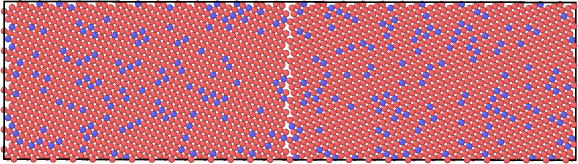
\includegraphics[width=0.70\textwidth]{configuration.png}
\caption{$\gamma$U-10Mo \{120\} symmetric tilt grain boundary at the initial configuration. Grain boundaries are in the middle and on the edges of the supercell. Red atoms are uranium and blue atoms are molybdenum.}
\label{fig:gb}
\end{figure}

The dimensions of the supercells are at least $50 \text{ \r{A}} \times 200 \text{ \r{A}} \times 50 \text{ \r{A}}$, with the dimension perpendicular to the GB being the longest. These systems are verified to be large enough to obtain a stable system, from which converged energies can be extracted \cite{beeler2018}. A single simulation consists of 35000 to 50000 atoms depending on the type and misorientation angle of the GB. A temperature range starting from 600 K to 1200 K has been probed with an increment of 100 K. Three different compositions are investigated for symmetric tilt GB systems: $\gamma$U-7Mo, $\gamma$U-10Mo, and $\gamma$U-12Mo (in weight percent). For asymmetric tilt and twist GBs, only $\gamma$U-10Mo has been considered. For any single GB at a given temperature, five simulations are performed with different random number seeds. This allows for the evaluation of the statistical significance of the results since the seeds determine the initial distribution of Mo atoms and the velocities of both the U and Mo atoms in the supercell.

An initial validation study was performed to ensure the correct construction of the GBs, measured against the reproducibility of GB energies in the literature. After validating the structures of GB systems, simulations are performed to extract the diffusion coefficients in the GBs. To that end, the supercells are first relaxed in an NPT ensemble using a Nose-Hoover thermostat and barostat with a damping parameter of 0.1 ps. 100,000 steps are performed with a timestep of 1 fs, making the NPT relaxation 100 ps in length. Afterward, the simulation box lengths are fixed at the equilibrated supercell lengths obtained during the NPT relaxation and the systems are further equilibrated for 100 ps in an NVT ensemble. The NVT ensemble also uses a Nose-Hoover thermostat with a 0.1 ps damping parameter. The production simulations are then executed for 5,000,000 steps with a timestep of 2 fs, yielding a 10 ns trajectory for the determination of diffusion coefficients.

To examine the diffusion of Xe in $\gamma$U-Mo GBs, the $\gamma$U-10Mo symmetric tilt GBs are generated as per the prior procedure, but with a single Xe substitutional defect inserted in both GBs (a total of two Xe atoms in the system). For Xe simulations, the 100 ps NPT-ensemble relaxation and a subsequent 50 ps NVT-ensemble relaxation are first performed, then Xe substitutions are made. After Xe insertion, the system is again relaxed in an NVT ensemble for 50 ps. A timestep of 1 fs is used throughout the relaxation period. Afterward, a 100 ns data collection period begins with a timestep of 5 fs. Since there are only two Xe atoms per system and Xe diffusion is slower than either U or Mo diffusion \cite{park2023}, collecting data over a longer period of time is necessary for diffusion calculations.

To calculate the mean squared displacement (MSD) of the U, Mo, and Xe atoms in the GB, a buffer averaging scheme is deployed as described in \cite{rapaport2004}. In this scheme, multiple parallel MSD calculations are performed over subsets of the full simulations. For example, in the case of systems without Xe, the first buffer computes the MSD from 2 ns to 7 ns, and the second computes MSD from 3 ns to 8 ns, and so on. MSD values from 4 such buffers are then averaged. While the average from only 4 buffers is enough to get a smooth MSD versus time curve of U and Mo atoms, MSD calculations of Xe need more buffers. Therefore, a total of 34 buffers, where each buffer calculates the MSD over 12.5 ns, are employed for the systems with Xe. The starting times of two successive buffers are separated by 2.5 ns in this case. Once the buffer-averaged MSD values are available as a function of time, the Einstein relation can be used to compute the diffusion coefficients. The diffusion coefficients in the GB can then be calculated from Eq. \ref{eq:ein}:

\begin{align}\label{eq:ein}
	D_{GB} &= \frac{1}{2\xi} \frac{d \langle r^2 \rangle_{GB}}{dt}
\end{align}
where $\xi$ is the dimensionality of the diffusion and $\langle r^2 \rangle_{GB}$ is the MSD of the atoms in the GB. The diffusion coefficients for all the aforementioned systems are calculated using this equation. Since the studied systems are two-dimensional GBs, the dimensionality is $\xi=2$. Generally, diffusion follows the Arrhenius equation as formulated in Eq. \ref{eq:arrD}:
\begin{align}
	\label{eq:arrD}
	D &= D_0 \exp \bigg( -\frac{E_a}{k_B T} \bigg)
\end{align}
where $D_0$ is the pre-exponential factor, $E_a$ is the activation energy, $T$ is the absolute temperature, and $k_B$ is the Boltzmann constant. Arrhenius fits are calculated for the diffusion coefficients of all the simulated systems.


\section{Results}

\subsection{Grain boundary validation}

To check the validity of the constructed systems, GB energies for $\gamma$U-10Mo GBs are calculated to compare against literature values. The systems are relaxed over 100 ps in an NPT ensemble at 1200 K, with energies averaged over the final 50 ps, with 25 unique simulations performed for each GB system. The symmetric tilt GB energies are shown in Figure \ref{fig:gbe}, with the error bars indicating $1\sigma$ confidence intervals. All symmetric tilt GB energies are within $2\sigma$ of the values reported in Beeler et al. \cite{beeler2018}. Therefore, the computed GB energies in this work agree with the results from Beeler et al. It should be noted that the GB systems used by Beeler et al. have roughly 10 times fewer atoms. The average GB energy for the examined symmetric tilt GBs is 0.68 Jm$^{-2}$.

\begin{figure}[!ht]
\centering
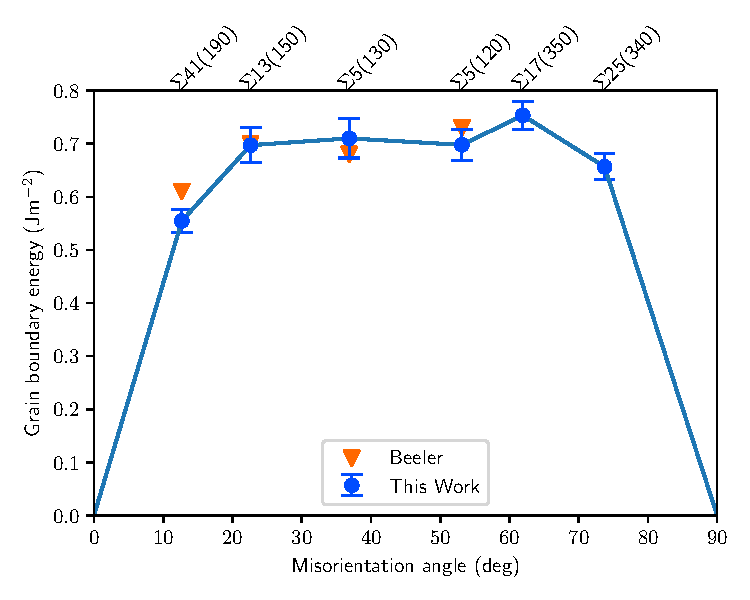
\includegraphics[width=0.70\textwidth]{gbe.pdf}
\caption{Grain boundary energies as a function of misorientation angle for $\gamma$U-10Mo symmetric tilt grain boundaries at 1200 K.}
\label{fig:gbe}
\end{figure}

Novel asymmetric tilt and twist GBs are explored in this work which have not been studied previously. The energies of these GBs in $\gamma$U-10Mo are shown in Table \ref{tab:gbe}. The average GB energy is 0.90 Jm$^{-2}$ for the probed asymmetric tilt and twist GB systems. With the exception of the asymmetric \{190\} tilt GB, all the asymmetric tilt and twist GBs have higher GB energy than the symmetric tilt GBs. This means the asymmetric tilt and twist GBs are generally energetically less favorable to form than the symmetric tilt GBs.

\begin{table}[!ht]
\centering
\caption{Grain boundary energies of $\gamma$U-10Mo asymmetric tilt and twist grain boundaries at 1200 K.}
\label{tab:gbe}
\begin{tabular}{lc}
\toprule
GB plane & Energy (Jm$^{-2}$) \\
\midrule
asym \{110\} & 0.77 \\
asym \{130\} & 1.15 \\
asym \{190\} & 0.41 \\
asym \{350\} & 1.10 \\
twist \{110\} & 0.84 \\
twist \{230\} & 1.14 \\
\bottomrule
\end{tabular}
\end{table}


\FloatBarrier
\subsection{Temperature-dependent GB width}\label{sec:res1}

In order to correctly identify the GB diffusion, the number of GB atoms, often approximated using the GB width, needs to be determined. Figure \ref{fig:hist} shows the histogram of the squared displacements of all atoms. Atoms with a squared displacement of less than $3$ \r{A}$^2$ are assumed to be vibrating about their lattice positions, and not contributing to the net diffusion. In the systems with a GB, this comprises the majority of atoms in the system. The second peak of the histogram appears at $9$ \r{A}$^2$, which is close to the square of the average nearest neighbor distance in U-10Mo (around $3$ \r{A}). Other peaks are found also at squares of multiples of the nearest neighbor distance. OVITO is used to visually inspect the atoms having more than $3$ \r{A}$^2$ squared displacement \cite{ovito}. Through the inspection of atomic trajectories, it is confirmed that these atoms constitute the GBs in the system. Thus, the sum of the squared displacement of atoms having more than $3$ \r{A}$^2$ squared displacement is equivalent to the total squared displacement of the GB atoms. GB MSD can then be determined from that displacement by averaging over the number of atoms that are participating in the diffusion process.

\begin{figure}[!ht]
\centering
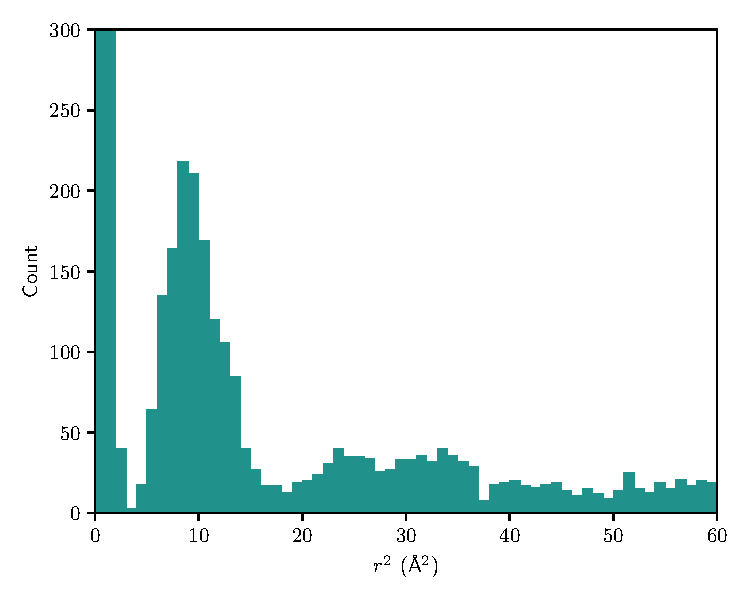
\includegraphics[width=0.60\textwidth]{histogram.pdf}
\caption{Histogram of squared displacements of atoms in a $\gamma$U-10Mo simulation at 1200 K. The histogram bars on the domain x$\in$[0,2] are curtailed to better illustrate the data.}
\label{fig:hist}
\end{figure}

The number of diffusing atoms is plotted against inverse temperature for the symmetric tilt \{120\} GB in U-10Mo in Figure \ref{fig:atomVsT}. The simulation box for this orientation has 36,864 total atoms. It is observed that the number of diffusing GB atoms increases with increasing temperature. The percentage of atoms participating in diffusion rises from $0.7\%$ at 600 K to $12.7\%$ at 1200 K. This increase is almost exponential in nature. This correlates physically to an effective GB width that increases from 0.1 nm at 600 K to 1.4 nm at 1200 K. The effective GB width is calculated using the formula $w = \frac{DA}{TA} \frac{L_y}{2}$, where $DA$ and $TA$ are the number of diffusing atoms and the number of total atoms in the system, respectively, and $L_y$ is the length of the supercell in the direction perpendicular to the GBs. $L_y$ is divided by two due to the two GBs present in the supercell. The effective GB width defined here is similar to the notion of diffusional width as described in \cite{keblinski1999}. The result here depicts that assuming a fixed GB width across temperatures, as it has been done for U$_3$Si$_2$ \cite{cooper2021}, would have been erroneous for the U-Mo system.

\begin{figure}[!ht]
\centering
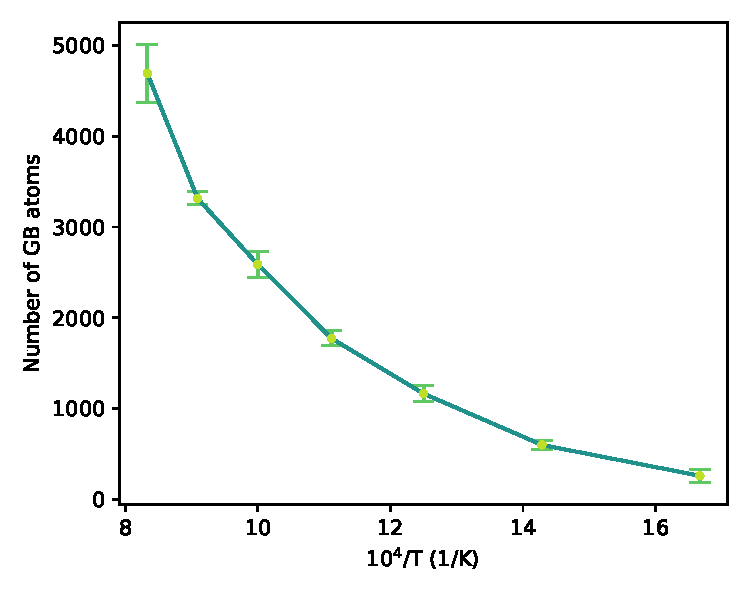
\includegraphics[width=0.60\textwidth]{atomsVsT.pdf}
\caption{Number of grain boundary atoms as a function of temperature for symmetric tilt \{120\} in $\gamma$U-10Mo.}
\label{fig:atomVsT}
\end{figure}


\FloatBarrier
\subsection{Total diffusion coefficients}

The total diffusion coefficients of various symmetric tilt GBs in $\gamma$U-10Mo are shown in Figure \ref{fig:u10mo}(a). The diffusion behavior is generally Arrhenius, and the spread in diffusion coefficients due to tilt angles is within one order of magnitude, regardless of the temperature. The order of magnitude of diffusion coefficients ranges from $10^{-11}$ m$^2$s$^{-1}$ in the high-temperature region to $10^{-12}$ m$^2$s$^{-1}$ in the low-temperature region. The standard deviation of diffusion coefficients at 1200 K is around $10^{-12}$ m$^2$s$^{-1}$ on average, while at 600 K it is around $10^{-13}$ m$^2$s$^{-1}$ on average, with the standard deviation monotonically increasing with temperature. Error bars are excluded from the figure for readability. The pre-exponential factors and activation energies from the Arrhenius fits are listed in Table \ref{tab:u10moArr}. The table lists values for U GB diffusion, Mo GB diffusion, and total GB diffusion. The activation energy for total diffusion is about 0.2-0.3 eV for the examined GBs in $\gamma$U-10Mo. This energy can be compared to the migration energies of point defect diffusion in $\gamma$U-10Mo. A recent study by Park et al. reports the migration energies of interstitial and vacancy diffusion of U in $\gamma$U-10Mo to be 0.40 eV and 0.73 eV, respectively \cite{park2023}. The activation energy of diffusion in the GB being lower than the migration energies of point defects indicates that the GB diffusion is not solely mediated by the migration of point defects. It also suggests that the GBs in $\gamma$U-Mo have highly disordered regions, where discernible point defects might be nonexistent.

\begin{figure}[!ht]
\begin{subfigure}{\textwidth}
	\centering
	\caption{}
	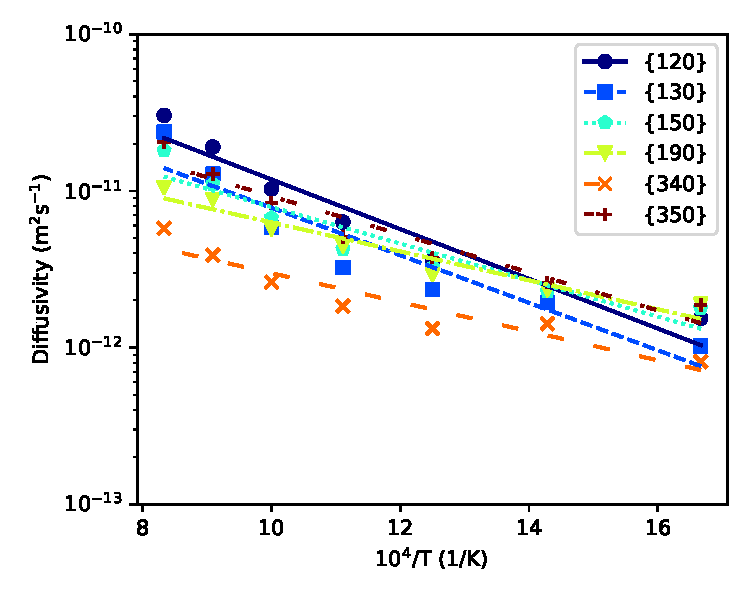
\includegraphics[width=0.65\textwidth]{u10mo_lin.pdf}
\end{subfigure}

\begin{subfigure}{\textwidth}
	\centering
	\caption{}
	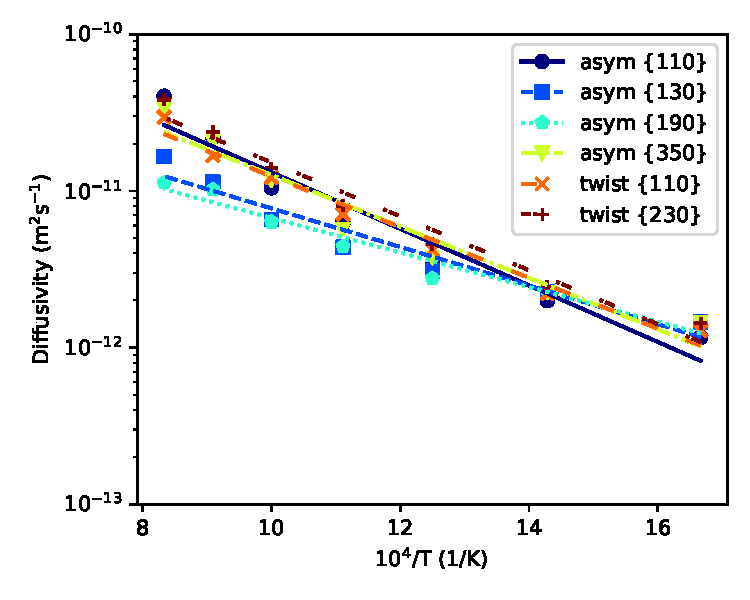
\includegraphics[width=0.65\textwidth]{asym_twist_lin.pdf}
\end{subfigure}
\caption{Total diffusivity in (a) symmetric tilt grain boundaries and (b) asymmetric tilt and twist grain boundaries for $\gamma$U-10Mo as a function of inverse temperature. Solid and dashed lines are Arrhenius fits to the data points.}
\label{fig:u10mo}
\end{figure}

\begin{table}[!ht]
\centering
\caption{Prefactors and activation energies for the Arrhenius equation fits for various symmetric tilt grain boundaries in $\gamma$U-10Mo.}
\label{tab:u10moArr}
\begin{tabular}{lllllll}
\toprule
GB plane & $D_{0,gb}^U$      & $E_{a,gb}^U$
	 & $D_{0,gb}^{Mo}$   & $E_{a,gb}^{Mo}$
	 & $D_{0,gb}^{Tot}$  & $E_{a,gb}^{Tot}$ \\
\midrule
\{120\} & 5.39 $\times 10^{-10}$ & 0.322
        & 1.35 $\times 10^{-10}$ & 0.271
        & 4.56 $\times 10^{-10}$ & 0.315  \\
\{130\} & 2.95 $\times 10^{-10}$ & 0.308
        & 8.06 $\times 10^{-11}$ & 0.242
        & 2.56 $\times 10^{-10}$ & 0.301  \\
\{150\} & 1.38 $\times 10^{-10}$ & 0.239
        & 2.92 $\times 10^{-11}$ & 0.173
        & 1.15 $\times 10^{-10}$ & 0.231  \\
\{190\} & 5.94 $\times 10^{-11}$ & 0.187
        & 2.13 $\times 10^{-11}$ & 0.161
        & 5.27 $\times 10^{-11}$ & 0.183  \\
\{340\} & 2.72 $\times 10^{-11}$ & 0.186
        & 1.39 $\times 10^{-11}$ & 0.176
        & 2.53 $\times 10^{-11}$ & 0.184  \\
\{350\} & 1.79 $\times 10^{-10}$ & 0.248
        & 4.58 $\times 10^{-11}$ & 0.197
        & 1.51 $\times 10^{-10}$ & 0.241  \\
\bottomrule
\end{tabular}
\end{table}

The diffusion coefficients for asymmetric tilt and twist GBs in $\gamma$U-10Mo are depicted in Figure \ref{fig:u10mo}(b). The variance in the diffusion coefficient with respect to orientation is very minor, and less than that for symmetric tilt GBs. The magnitude of the diffusivity for non-symmetric tilt GBs is in the same range as the symmetric tilt systems. Thus, the overall impact of the orientation of GBs on the diffusivity appears to be minimal. The data in Figure \ref{fig:u10mo}(b) still show a general Arrhenius trend, and the prefactors and activation energies for these systems are tabulated in Table \ref{tab:asym} in the appendix. The standard deviation in these systems is approximately $2.8 \times 10^{-12}$ m$^2$s$^{-1}$ at 1200 K, and $2.8 \times 10^{-13}$ m$^2$s$^{-1}$ at 600 K. The general errors for all systems are sufficiently small that the trends with respect to temperature are statistically significant.

The orientation-averaged values for $\gamma$U-7Mo, $\gamma$U-10Mo, and $\gamma$U-12Mo are shown in Figure \ref{fig:comp}. While not shown, the range of diffusivities with respect to misorientation angles in different compositions is also within one order of magnitude, and thus only orientation-averaged diffusivities are displayed. From the figure, it can be noticed that the diffusivity is negatively correlated with the Mo content of the fuel. This is somewhat expected as the U self-diffusivity is higher than that of Mo \cite{huang2013}, and increased Mo content suppresses self-diffusivity in $\gamma$U-Mo. The general trend as a function of the temperature of the diffusivity for the three examined compositions is identical. The standard deviations for the U-7Mo and U-12Mo systems are comparable to that of U-10Mo, which indicates that the trend observed with composition is statistically significant. Table \ref{tab:compArr} provides the Arrhenius parameters for the different compositions. Also, the total GB diffusion coefficients for different tilts and temperatures in $\gamma$U-7Mo and $\gamma$U-12Mo are listed in Tables \ref{tab:u7mo} and \ref{tab:u12mo} of the appendix for completeness.

\begin{figure}[!ht]
\centering
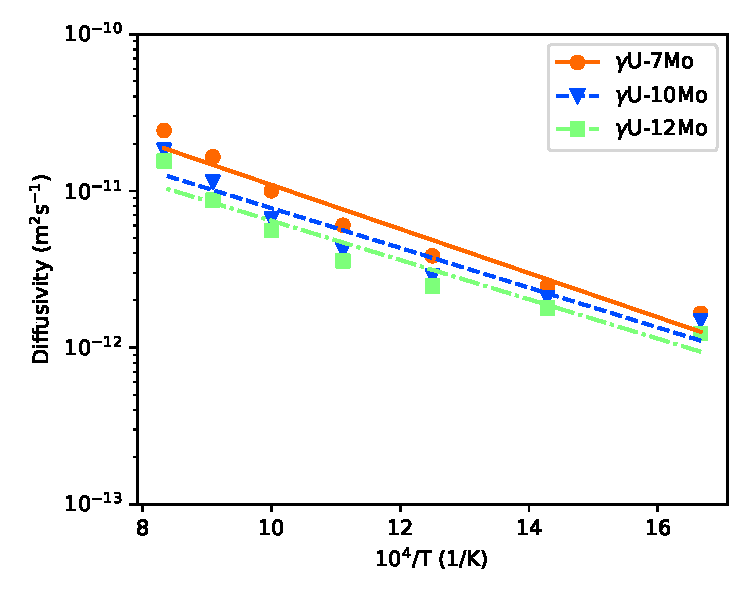
\includegraphics[width=0.70\textwidth]{composition_lin.pdf}
\caption{Grain boundary orientation-averaged diffusion coefficients for $\gamma$U-7Mo, $\gamma$U-10Mo, and $\gamma$U-12Mo.}
\label{fig:comp}
\end{figure}

\begin{table}[!ht]
\centering
\caption{Prefactors and activation energies for the Arrhenius equation fits for grain boundary diffusion in $\gamma$U-Mo alloys.}
\label{tab:compArr}
\begin{tabular}{lllllll}
\toprule
Composition & $D_{0,gb}^U$      & $E_{a,gb}^U$
	    & $D_{0,gb}^{Mo}$   & $E_{a,gb}^{Mo}$
	    & $D_{0,gb}^{Tot}$  & $E_{a,gb}^{Tot}$ \\
\midrule
$\gamma$U-7Mo  & 3.12 $\times 10^{-10}$ & 0.284 & 7.43 $\times 10^{-11}$
	       & 0.231 & 2.78 $\times 10^{-10}$ & 0.279  \\
$\gamma$U-10Mo & 1.68 $\times 10^{-10}$ & 0.258 & 4.65 $\times 10^{-11}$
	       & 0.210 & 1.44 $\times 10^{-10}$ & 0.252  \\
$\gamma$U-12Mo & 1.38 $\times 10^{-10}$ & 0.256 & 4.03 $\times 10^{-11}$
	       & 0.206 & 1.16 $\times 10^{-10}$ & 0.249  \\
\bottomrule
\end{tabular}
\end{table}


\FloatBarrier
\subsection{Species diffusion coefficients}

The orientation-averaged U, Mo, and Xe GB diffusion coefficients are displayed in Figure \ref{fig:umoxe}. At high temperatures, all three species show GB diffusivity of the same order of magnitude. For all examined temperatures, U GB diffusivity is roughly double the GB diffusivity of Mo. The difference between the Xe GB diffusion coefficient and the U and Mo GB diffusion coefficients increases with decreasing temperature. Around 600 K, the Xe GB diffusion coefficient is approximately two orders of magnitude lower than that of U and Mo.

\begin{figure}[!ht]
\centering
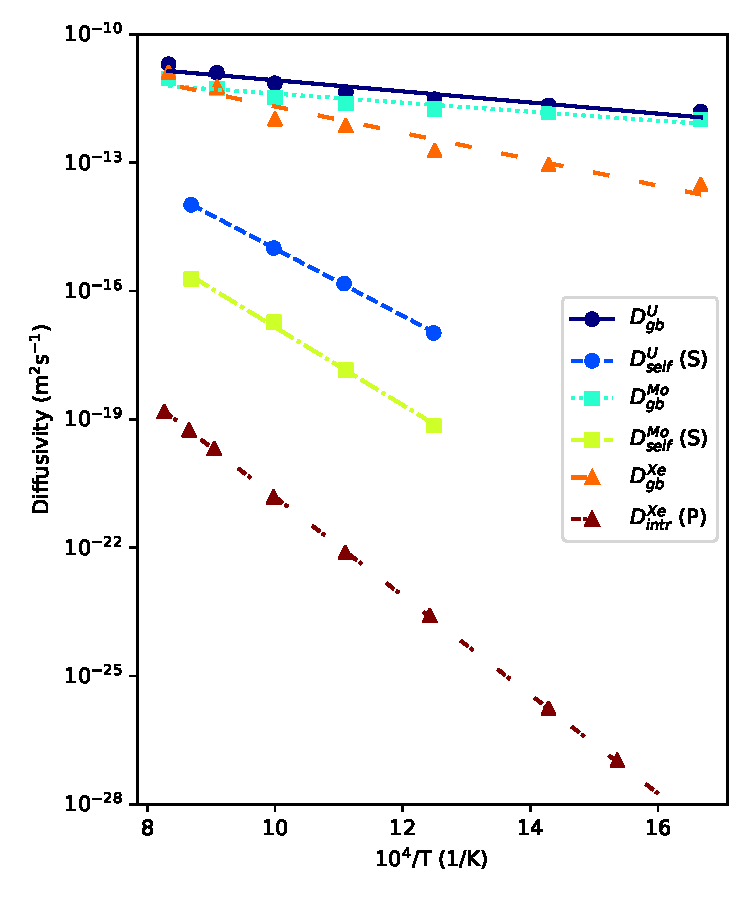
\includegraphics[width=0.80\textwidth]{comparison4.pdf}
\caption{Orientation-averaged U, Mo, and Xe grain boundary diffusivities in $\gamma$U-10Mo with literature data. S represents the U and Mo self diffusivity in $\gamma$U-9Mo from Smirnova et al. \cite{smirnova2015}. P represents the intrinsic diffusivity of Xe in $\gamma$U-10Mo from Park et al. \cite{park2023}.}
\label{fig:umoxe}
\end{figure}

Additional literature data on self-diffusivities in $\gamma$U-9Mo from Smirnova et al. \cite{smirnova2015} is included in Figure \ref{fig:umoxe} to provide perspective. These self-diffusivities were computed using the same ADP potential used for this work. Since the GB diffusivities of $\gamma$U-7Mo and $\gamma$U-10Mo are close, the difference in composition between the studies is not significant enough to prevent a comparison. The GB diffusion coefficient of U is about three orders of magnitude higher than the self-diffusion coefficient at high temperatures. The difference between GB diffusivity and self-diffusivity grows larger with decreasing temperature. At around 800 K, the difference is about five orders of magnitude. For Mo, the GB diffusion coefficient is about four orders of magnitude higher than the self-diffusion coefficient at high temperatures, while the difference spans seven orders of magnitude around 800 K. The intrinsic diffusion coefficient of Xe from Park et al. \cite{park2023} is included in the figure as well. This intrinsic diffusion coefficient was calculated using an EAM potential of U-Mo-Xe \cite{smirnova2013}. The difference between GB diffusion and intrinsic diffusion of Xe is more drastic than U and Mo. At high temperatures, the GB diffusion coefficient of Xe is about seven orders of magnitude higher than the intrinsic diffusion coefficient of Xe, while at 800 K, this enlarges to a difference of about ten orders of magnitude. Table \ref{tab:enhance} summarizes the species-wise diffusion enhancements by GBs at four different temperatures. It is apparent from the table that the diffusion enhancement is larger at lower temperatures. This means the overall diffusion in the material is dominated mostly by GB diffusion at lower temperatures, and thus GB diffusion is more important in the calculation of the effective diffusivity of the material. The diffusion enhancement starts to wane at higher temperatures since the activation energy of GB diffusion is lower than that of bulk diffusion. This difference in activation energies is expected and is observable in Figure \ref{fig:umoxe}. Species-specific diffusion prefactors and activation energies are included in Tables \ref{tab:u10moArr}, \ref{tab:compArr}, \ref{tab:compArrHigh}, \ref{tab:compArrLow}, \ref{tab:u7mo}, \ref{tab:asym}, \ref{tab:u12mo}, and \ref{tab:xe}. 

\begin{table}[!ht]
\centering
\caption{Ratio of grain boundary diffusivity and self/intrinsic diffusivity.}
\label{tab:enhance}
\begin{tabular}{lllllll}
\toprule
Temp   & $D^U_{gb}/D^U_{self}$
       & $D^{Mo}_{gb}/D^{Mo}_{self}$
       & $D^{Xe}_{gb}/D^{Xe}_{intr}$ \\
\midrule
600 K  & 2.76 $\times 10^8$ & 8.30 $\times 10^{10}$ & 1.01 $\times 10^{15}$ \\
800 K  & 2.85 $\times 10^5$ & 2.38 $\times 10^7$    & 9.62 $\times 10^{10}$ \\
1000 K & 7.33 $\times 10^3$ & 2.34 $\times 10^5$    & 6.85 $\times 10^8$  \\
1200 K & 1.00 $\times 10^3$ & 1.96 $\times 10^4$    & 9.85 $\times 10^7$  \\
\bottomrule
\end{tabular}
\end{table}


\FloatBarrier
\subsection{Dependence of diffusion on misorientation angle}

The effect of misorientation angle on diffusion is shown in Figure \ref{fig:dvstilt}. Figure \ref{fig:dvstilt}(a) shows the GB diffusivity of the species against misorientation angle in $\gamma$U-10Mo at 800 K. Figure \ref{fig:dvstilt}(b) shows similar results but at 1200 K. Since these are bcc structures, having a 90$^{\circ}$ tilt means it is a perfect lattice without any GBs. GBs having a misorientation angle of less than 15 degrees (or more than 75 degrees) are defined as low-angle GBs (LAGB) and those having more than 15 degrees (or less than 75 degrees) of misorientation are defined as high-angle GBs (HAGB) for the purpose of this discussion. It is observed that LAGBs have slightly lower diffusivities than HAGBs. At low temperatures, all HAGBs have similar diffusivities, and the effect of misorientation on these boundaries is not pronounced, with the exception of the \{130\} GB. The symmetric tilt \{130\} GB might be a special boundary and additional simulations would likely be required to verify the exception. At high temperatures, the amount of misorientation affects both LAGBs and HAGBs. The greater the misorientation, the greater the diffusivity. It is to be emphasized that misorientation angles $\theta$ and $90-\theta$ are the same because of the inherent symmetry in bcc structures.

\begin{figure}[!ht]
    \centering
    \begin{subfigure}{0.49\textwidth}
        \centering
        \caption{}
        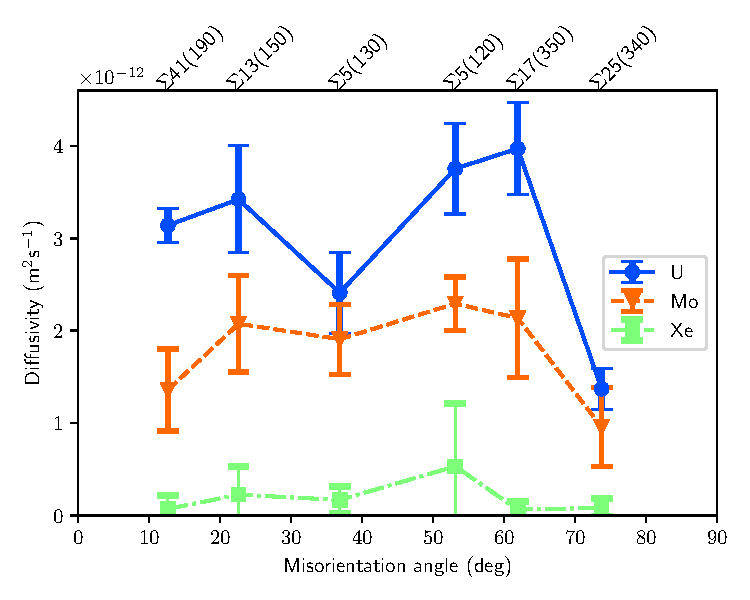
\includegraphics[width=\textwidth]{DvsTilt_10mo_2.pdf}
    \end{subfigure}
    \begin{subfigure}{0.49\textwidth}
        \centering
        \caption{}
        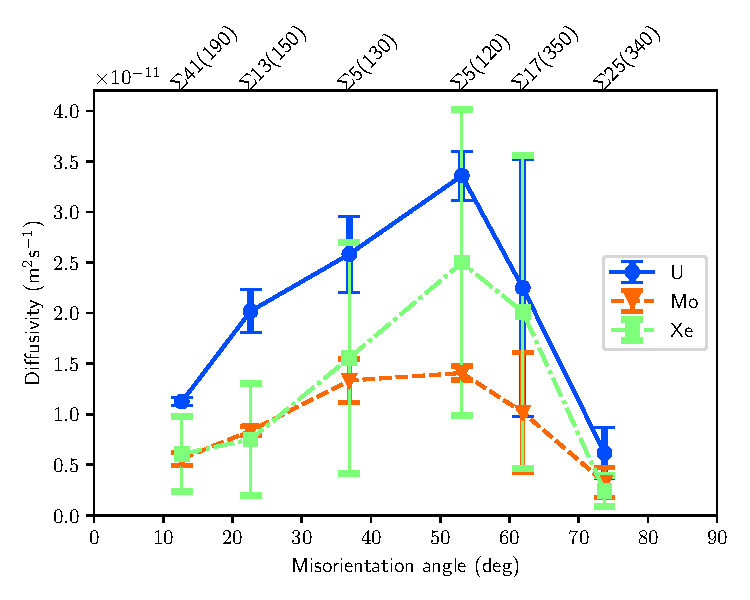
\includegraphics[width=\textwidth]{DvsTilt_10mo.pdf}
    \end{subfigure}
\caption{Diffusivities for U, Mo, and Xe with respect to misorientation angles for $\gamma$U-10Mo at (a) 800 K, and (b) 1200 K.}
\label{fig:dvstilt}
\end{figure}

There do not appear to be any species-specific trends from the misorientation angle, as all species generally diffuse faster at higher temperatures, and tend to diffuse slightly faster with misorientation angles between 30$^{\circ}$ and 65$^{\circ}$. For all examined misorientation angles at low temperatures, the following trend seems to be true in general:
\begin{align}
	D_{gb}^U > D_{gb}^{Mo} > D_{gb}^{Xe}
\end{align}
However, this trend tends to break down at high temperatures where D$_{gb}^{Xe}$ becomes comparable to that for U and Mo. It can also be seen that the Xe diffusion coefficients have a larger relative variance compared to the other two species. This is expected since we only compute properties from the diffusion of 2 Xe atoms per simulation. In contrast, we have thousands of U and Mo atoms per simulation.


\FloatBarrier
\section{Discussion}

\subsection{Nature of diffusion}

GBs can be interpreted as collections of dislocations and a pure tilt GB is essentially an array of parallel edge dislocations. Analysis of the atomistic simulations performed in this work reveals dislocation pipe diffusion in symmetric tilt LAGBs, and this diffusion is mostly one-dimensional where the diffusion pipes are parallel to the tilt axis. The atomic trajectories in a cross-sectional GB view and the directional MSDs of the symmetric tilt \{190\} are provided in Figure \ref{fig:190}. Subfigures \ref{fig:190}(a) and \ref{fig:190}(b) are at 700 K, and \ref{fig:190}(c) and \ref{fig:190}(d) are at 1100 K. The cross-sections reveal the diffusion pipes. Diffusion outside these pipes is not prominent even if the atoms are within the GB plane. This explains why the effective GB width as defined in section \ref{sec:res1} can sometimes be less than the lattice parameter, as not all atoms at the GB are participating in the diffusion. The MSDs in the direction perpendicular to the GB plane (y-axis), and in the direction perpendicular to the tilt axis but parallel to the GB plane (x-axis) are similar in magnitude. Thus, it can be stated that the diffusion in the symmetric tilt \{190\} GB is primarily happening in the direction of the tilt axis.

\begin{figure}[!ht]
\centering
	\begin{subfigure}{0.49\textwidth}
		\centering
		\caption{}
		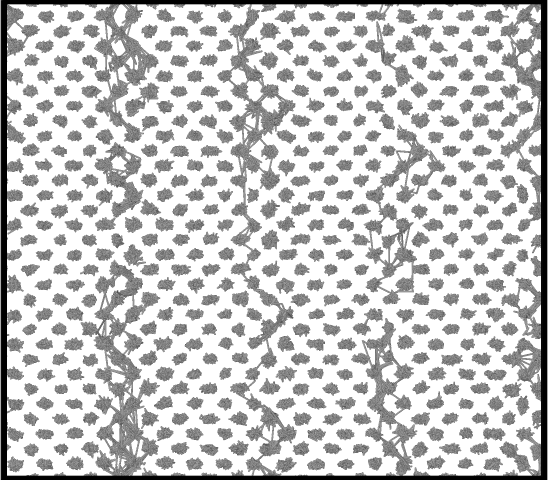
\includegraphics[height=5cm]{190at700cs.png}
	\end{subfigure}
	\begin{subfigure}{0.49\textwidth}
		\centering
		\caption{}
		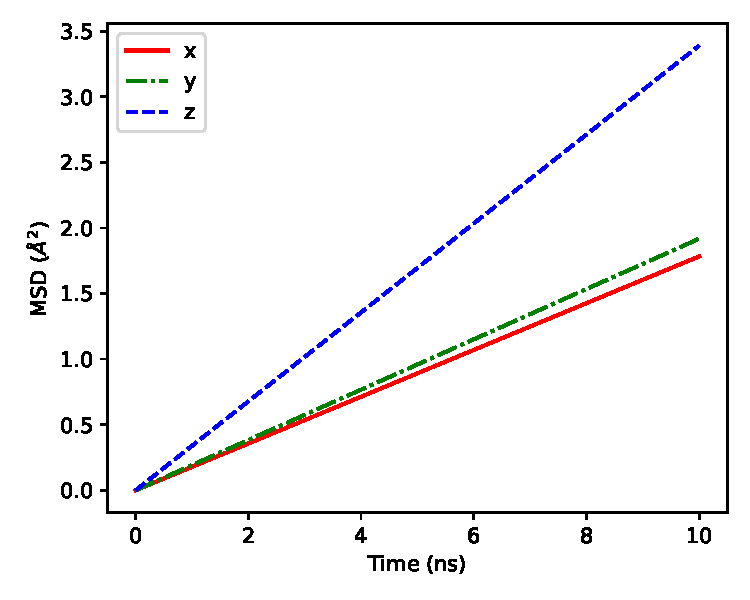
\includegraphics[height=5cm]{190at700xyz.pdf}
	\end{subfigure}
    \par\medskip
	\begin{subfigure}{0.49\textwidth}
		\centering
		\caption{}
		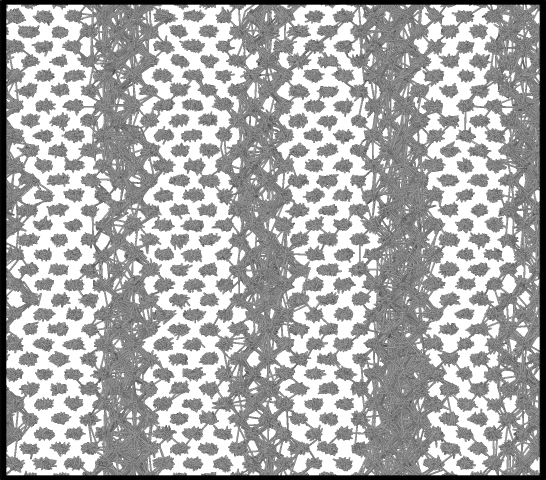
\includegraphics[height=5cm]{190at1100cs.png}
	\end{subfigure}
	\begin{subfigure}{0.49\textwidth}
		\centering
		\caption{}
		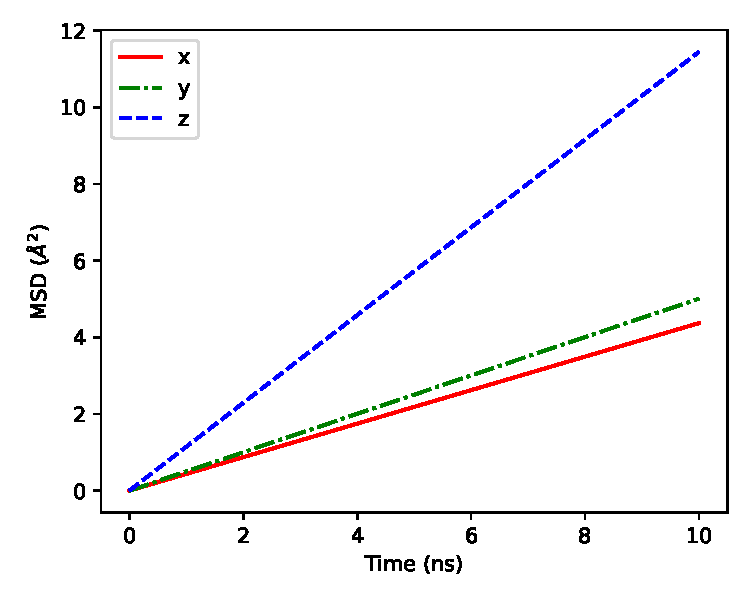
\includegraphics[height=5cm]{190at1100xyz.pdf}
	\end{subfigure}
\caption{Atomic trajectory lines in the GB cross sections at (a) 700 K and (c) 1100 K, and the MSD at (b) 700 K and (d) 1100 K for the symmetric tilt \{190\} grain boundary.}
\label{fig:190}
\end{figure}

Figure \ref{fig:130} displays the atomic trajectories and the directional MSDs for the symmetric tilt \{130\} GB. Contrary to the \{190\} system, the diffusion in \{130\} is two-dimensional. The diffusion on the GB plane does not have any directional preference in this case. This is true for most HAGBs. For some configurations, such as the \{340\} system (misorientation angle of 16.3 degrees), the diffusion behavior can be somewhere in between. In those cases, the diffusion parallel to the tilt axis is significantly stronger than the diffusion perpendicular to the tilt axis (and parallel to the GB plane), which in turn is significantly stronger than the diffusion perpendicular to the GB plane. Thus, while the magnitude of diffusion is only marginally dependent upon the orientation of the GBs, the underlying nature of diffusion on symmetric tilt GBs can be substantially different, including 1-D or anisotropic effects, and such behaviors become more prevalent for LAGBs. 

\begin{figure}[!ht]
\centering
	\begin{subfigure}{0.49\textwidth}
		\centering
		\caption{}
		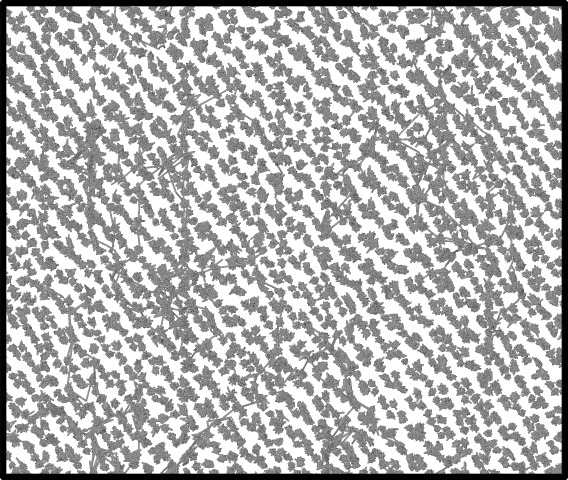
\includegraphics[height=5cm]{130at700cs.png}
	\end{subfigure}
	\begin{subfigure}{0.49\textwidth}
		\centering
		\caption{}
		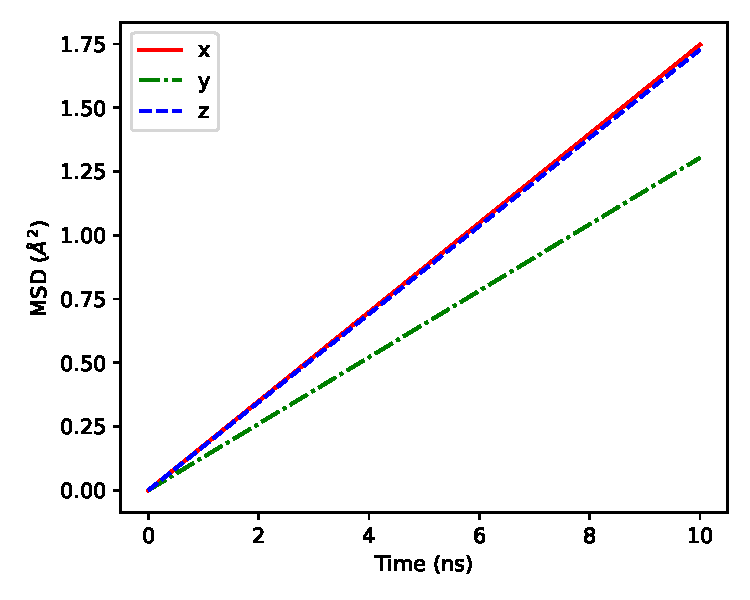
\includegraphics[height=5cm]{130at700xyz.pdf}
	\end{subfigure}
    \par\medskip
	\begin{subfigure}{0.49\textwidth}
		\centering
		\caption{}
		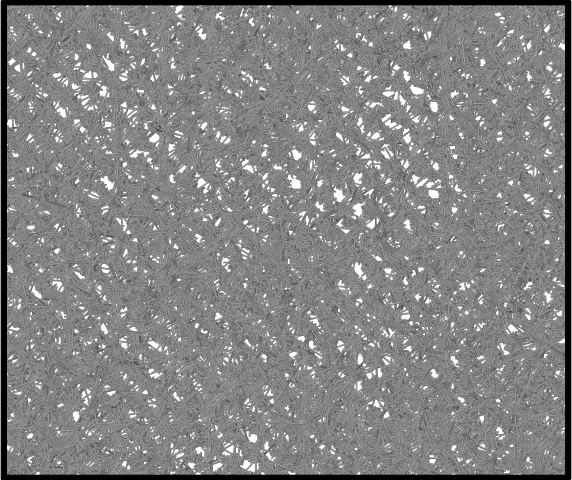
\includegraphics[height=5cm]{130at1100cs.png}
	\end{subfigure}
	\begin{subfigure}{0.49\textwidth}
		\centering
		\caption{}
		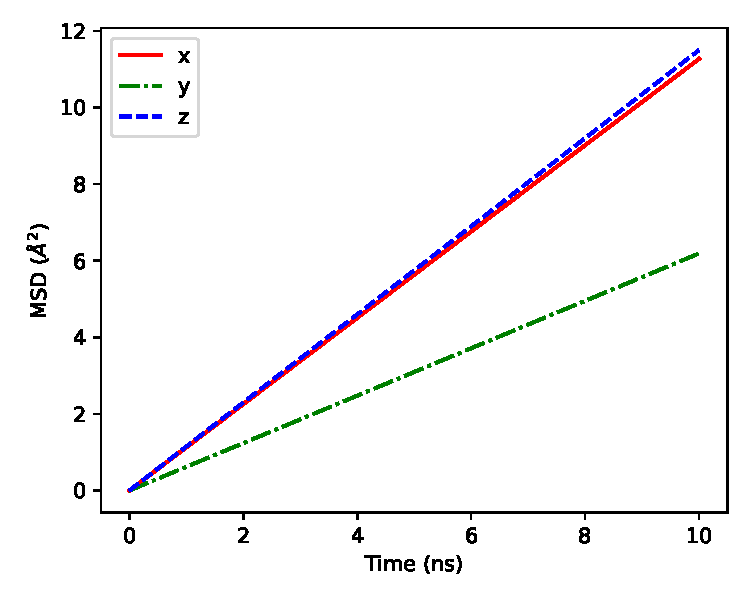
\includegraphics[height=5cm]{130at1100xyz.pdf}
	\end{subfigure}
\caption{Atomic trajectory lines in the GB cross sections at (a) 700 K and (c) 1100 K, and the MSD at (b) 700 K and (d) 1100 K for the symmetric tilt \{130\} grain boundary.}
\label{fig:130}
\end{figure}


\FloatBarrier
\subsection{Two diffusion regimes based on temperature}

The diffusion coefficients of $\gamma$U-Mo roughly follow the Arrhenius equation, but not exactly. The Arrhenius plot displays concavity for all configurations, indicating the possibility of sub-Arrhenius behavior. Similar behavior has been observed in U$_3$Si$_2$ fuel by Cooper et al. \cite{cooper2021}, but was neglected. Figure \ref{fig:2reg} shows the same data as in Figure \ref{fig:comp}, but separated into two different regimes: a high-temperature regime from 900 K to 1200 K and a low-temperature regime from 600 K to 800 K. A GB diffusion study by Suzuki et al. \cite{suzuki2005} describes this as heterophase fluctuations. The Arrhenius plots for Cu GB diffusion from Suzuki also show concavity, and they theorized this as a local melting event, where small embryos of liquid are supposed to exist for a short time before crystallizing into an ordered GB structure.

\begin{figure}[!ht]
\centering
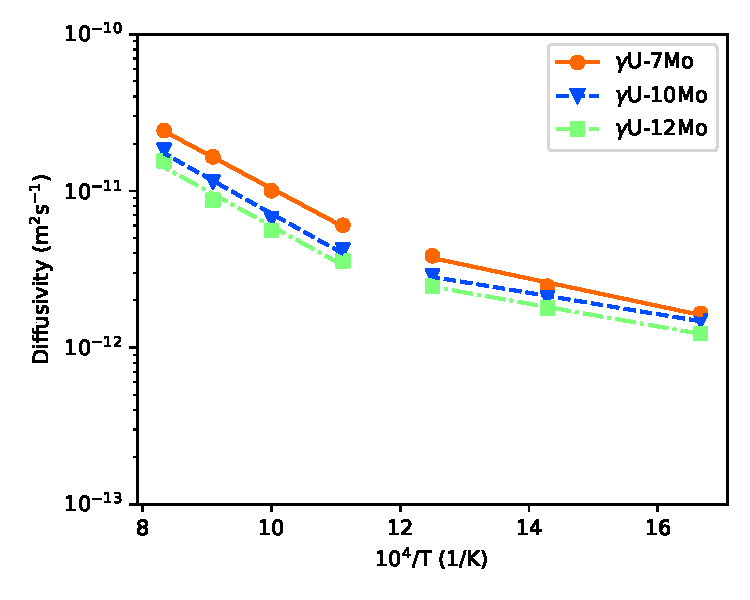
\includegraphics[width=0.60\textwidth]{2reg.pdf}
\caption{Arrehenius fits to two diffusion regimes.}
\label{fig:2reg}
\end{figure}

Arrhenius fits are thus applied separately for these two temperature regimes observed in Figure \ref{fig:2reg}, and prefactors and activation energies for these two regimes are provided in Tables \ref{tab:compArrHigh} and \ref{tab:compArrLow}. The activation energy for total GB diffusion is 0.457 eV for U-10Mo at high temperatures, which is 3.4 times higher than the activation energy at low temperatures (0.135 eV). We suggest the use of Arrhenius fits that are based on the two temperature regimes, e.g., to calculate the diffusion coefficient at 300 K, the low-temperature fit should be used. 

\begin{table}[!ht]
\centering
\caption{Prefactors and activation energies for the Arrhrenius equation fits for various compositions in the high-temperature regime.}
\label{tab:compArrHigh}
\begin{tabular}{lllllll}
\toprule
Composition & $D_{0,gb}^U$      & $E_{a,gb}^U$
	    & $D_{0,gb}^{Mo}$   & $E_{a,gb}^{Mo}$
	    & $D_{0,gb}^{Tot}$  & $E_{a,gb}^{Tot}$ \\
\midrule
$\gamma$U-7Mo  & 1.76 $\times 10^{-9}$ & 0.438 & 9.04 $\times 10^{-10}$
	       & 0.455 & 1.61 $\times 10^{-9}$ & 0.435  \\
$\gamma$U-10Mo & 1.76 $\times 10^{-9}$ & 0.468 & 4.47 $\times 10^{-10}$
	       & 0.412 & 1.45 $\times 10^{-9}$ & 0.457  \\
$\gamma$U-12Mo & 1.35 $\times 10^{-9}$ & 0.460 & 3.13 $\times 10^{-10}$
	       & 0.390 & 1.06 $\times 10^{-9}$ & 0.447  \\
\bottomrule
\end{tabular}
\end{table}

\begin{table}[!ht]
\centering
\caption{Prefactors and activation energies for the Arrhrenius equation fits for various compositions in the low-temperature regime.}
\label{tab:compArrLow}
\begin{tabular}{lllllll}
\toprule
Composition & $D_{0,gb}^U$      & $E_{a,gb}^U$
	    & $D_{0,gb}^{Mo}$   & $E_{a,gb}^{Mo}$
	    & $D_{0,gb}^{Tot}$  & $E_{a,gb}^{Tot}$ \\
\midrule
$\gamma$U-7Mo  & 5.08 $\times 10^{-11}$ & 0.177 & 1.12 $\times 10^{-11}$
	       & 0.119 & 4.61 $\times 10^{-11}$ & 0.173  \\
$\gamma$U-10Mo & 2.16 $\times 10^{-11}$ & 0.137 & 1.03 $\times 10^{-11}$
	       & 0.120 & 2.01 $\times 10^{-11}$ & 0.135  \\
$\gamma$U-12Mo & 2.12 $\times 10^{-11}$ & 0.145 & 1.11 $\times 10^{-11}$
	       & 0.129 & 1.96 $\times 10^{-11}$ & 0.143  \\
\bottomrule
\end{tabular}
\end{table}

These regimes may be due to different modes of diffusion that only get enabled at high temperatures, with the transition between the two diffusion regimes occurring at 800-900 K for this system. With additional thermal energy, given a fixed migration barrier, higher temperatures are more likely to overcome the energy barrier and induce diffusion. Given that 1) more atoms are participating in the diffusional process as temperature increases (Figure \ref{fig:atomVsT}), 2) diffusional pathways appear to become more varied at increasing temperature (Figure \ref{fig:130}), and 3) that the high-temperature diffusion regime exhibits a higher activation energy (Figure \ref{fig:2reg}), the assumption that increased temperature opens higher energy diffusional pathways seems reasonable. This may be an alternate way of viewing the same phenomena identified in Suzuki \cite{suzuki2005} and denoted as heterophase fluctuations. 


\FloatBarrier
\section{Conclusions}

In the present work, MD simulations are performed using an ADP potential to compute GB diffusion coefficients in $\gamma$U-Mo alloys \cite{starikov2018}. First, a way to distinguish the GB atoms is developed by individually identifying atoms that are participating in the GB diffusion process. It is observed that the number of GB atoms increases almost exponentially with temperature in the range of 600 K - 1200 K. The MSD of the GB atoms is then used to calculate the GB diffusivities of several $\gamma$U-Mo alloys ($\gamma$U-7Mo, $\gamma$U-10Mo, and $\gamma$U-12Mo) as a function of temperature and misorientation angle. GB diffusivities of U, Mo, and Xe are computed along with total GB diffusivity. The total GB diffusion is typically on the order of $10^{-12}$ to $10^{-11}$ m$^2$s$^{-1}$. The diffusivity is relatively insensitive to the misorientation angle, whereas there is a statistically significant negative correlation between the diffusivity and the concentration of Mo. Furthermore, the GB diffusion of U is generally faster than that of Mo, which is faster than that of Xe. The GB diffusion of U, Mo, and Xe are between three to fifteen orders of magnitude faster than the intrinsic/self-diffusion coefficients from literature, where GB diffusion becomes more dominant at lower temperatures. The GB diffusional acceleration is most prominent for Xe, which may dramatically impact the understanding of fission gas swelling behaviors. 

The diffusion coefficients obtained from this work can be used to model the mesoscale behavior of $\gamma$U-Mo fuels. The diffusivity values can also inform models of various creep mechanisms, such as Coble creep. Also, these values can be utilized to understand phenomena related to fuel performance, such as intergranular fission gas swelling.


\clearpage
\begin{appendices}

\setcounter{table}{0}
\renewcommand{\thetable}{A\arabic{table}}

\section{Diffusion coefficient tables}

\begin{table}[!ht]
\centering
\caption{Prefactors and activation energies for the Arrhenius equation fits for symmetric tilt grain boundaries in $\gamma$U-7Mo.}
\label{tab:u7mo}
\begin{tabular}{lllllll}
\toprule
GB plane & $D_{0,gb}^U$      & $E_{a,gb}^U$
	 & $D_{0,gb}^{Mo}$   & $E_{a,gb}^{Mo}$
	 & $D_{0,gb}^{Tot}$  & $E_{a,gb}^{Tot}$ \\
\midrule
\{120\}
	 & 9.43e-10 & 0.341
	 & 1.98e-10 & 0.284
	 & 8.32e-10 & 0.336 \\
\{130\}
	 & 5.28e-10 & 0.338
	 & 1.05e-10 & 0.245
	 & 4.51e-10 & 0.328 \\
\{150\}
	 & 3.02e-10 & 0.274
	 & 5.07e-11 & 0.198
	 & 2.67e-10 & 0.268 \\
\{190\}
	 & 6.36e-11 & 0.177
	 & 3.24e-11 & 0.182
	 & 6.05e-11 & 0.177 \\
\{340\}
	 & 5.55e-11 & 0.215
	 & 1.95e-11 & 0.190
	 & 5.20e-11 & 0.213 \\
\{350\}
	 & 4.15e-10 & 0.291
	 & 9.35e-11 & 0.242
	 & 3.70e-10 & 0.287 \\
\bottomrule
\end{tabular}
\end{table}

\begin{table}[!ht]
\centering
\caption{Prefactors and activation energies for the Arrhenius equation fits for asymmetric tilt and twist grain boundaries in $\gamma$U-10Mo.}
\label{tab:asym}
\begin{tabular}{lllllll}
\toprule
GB plane & $D_{0,gb}^U$      & $E_{a,gb}^U$
	 & $D_{0,gb}^{Mo}$   & $E_{a,gb}^{Mo}$
	 & $D_{0,gb}^{Tot}$  & $E_{a,gb}^{Tot}$ \\
\midrule
asym \{110\}
	& 1.00e-09 & 0.366
	& 2.76e-10 & 0.318
	& 8.41e-10 & 0.358 \\
asym \{130\}
	& 1.51e-10 & 0.250
	& 4.33e-11 & 0.204
	& 1.32e-10 & 0.244 \\
asym \{190\}
	& 9.32e-11 & 0.221
	& 3.99e-11 & 0.202
	& 8.53e-11 & 0.219 \\
asym \{350\}
	& 6.37e-10 & 0.330
	& 2.35e-10 & 0.308
	& 5.53e-10 & 0.326 \\
twist \{110\}
	& 6.24e-10 & 0.329
	& 1.60e-10 & 0.289
	& 5.16e-10 & 0.321 \\
twist \{230\}
	& 9.88e-10 & 0.351
	& 1.58e-10 & 0.278
	& 7.97e-10 & 0.341 \\
\bottomrule
\end{tabular}
\end{table}

\begin{table}[!ht]
\centering
\caption{Prefactors and activation energies for the Arrhenius equation fits for symmetric tilt grain boundaries in $\gamma$U-12Mo.}
\label{tab:u12mo}
\begin{tabular}{lllllll}
\toprule
GB plane & $D_{0,gb}^U$      & $E_{a,gb}^U$
	 & $D_{0,gb}^{Mo}$   & $E_{a,gb}^{Mo}$
	 & $D_{0,gb}^{Tot}$  & $E_{a,gb}^{Tot}$ \\
\midrule
\{120\}
	 & 3.87e-10 & 0.312
	 & 8.97e-11 & 0.248
	 & 3.18e-10 & 0.303 \\
\{130\}
	 & 4.94e-10 & 0.363
	 & 1.92e-10 & 0.323
	 & 4.29e-10 & 0.357 \\
\{150\}
	 & 1.02e-10 & 0.229
	 & 2.60e-11 & 0.169
	 & 8.48e-11 & 0.221 \\
\{190\}
	 & 5.92e-11 & 0.199
	 & 2.37e-11 & 0.177
	 & 5.26e-11 & 0.196 \\
\{340\}
	 & 1.50e-11 & 0.143
	 & 5.18e-12 & 0.098
	 & 1.31e-11 & 0.137 \\
\{350\}
	 & 1.35e-10 & 0.242
	 & 3.51e-11 & 0.186
	 & 1.11e-10 & 0.233 \\
\bottomrule
\end{tabular}
\end{table}

\begin{table}[!ht]
\centering
\caption{Xe diffusivities in $\gamma$U-10Mo symmetric tilt grain boundaries. Units are m$^2$/s.}
\label{tab:xe}
\begin{tabular}{ccccccc}
\toprule
GB plane & $D_{0,gb}^{Xe}$      & $E_{a,gb}^{Xe}$ \\
\midrule
\{120\} & 1.11e-08 & 0.677 \\
\{130\} & 1.46e-08 & 0.757 \\
\{150\} & 7.69e-10 & 0.532 \\
\{190\} & 4.78e-10 & 0.567 \\
\{340\} & 7.25e-11 & 0.425 \\
\{350\} & 4.42e-09 & 0.647 \\
\bottomrule
\end{tabular}
\end{table}

\end{appendices}


\FloatBarrier
\bibliographystyle{unsrt}
\bibliography{ref.bib}

\end{document}